%%%%%%%%%%%%%%%%%%%%%%%%%%%%%%%%%%%%%%%%%%%%%%%%%%%%%%%%%%%%%%%%%%%%%%%%%%%%%%%%%%
\begin{frame}[fragile]\frametitle{}
\begin{center}
{\Large Data Preparation}
\end{center}
\end{frame}

%%%%%%%%%%%%%%%%%%%%%%%%%%%%%%%%%%%%%%%%%%%%%%%%%%%%%%%%%%%%%%%%%%%%%%%%%%%%%%%%%%
\begin{frame}[fragile]\frametitle{Data}

Original input and output are in the form of polylines, meaning a list of points, each having x,y coordinates

\begin{center}
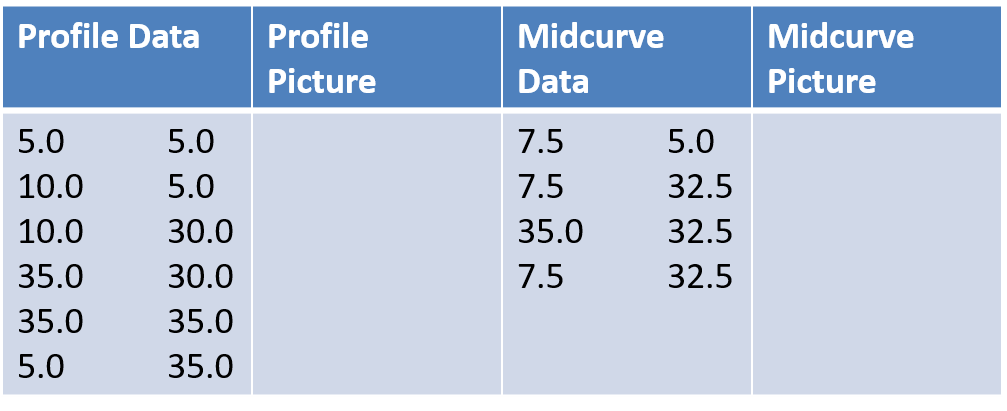
\includegraphics[width=0.9\linewidth,keepaspectratio]{midcurve27}
\end{center}	
\end{frame}

%%%%%%%%%%%%%%%%%%%%%%%%%%%%%%%%%%%%%%%%%%%%%%%%%%%%%%%%%%%%%%%%%%%%%%%%%%%%%%%%%%
\begin{frame}[fragile]\frametitle{Data}
\begin{center}
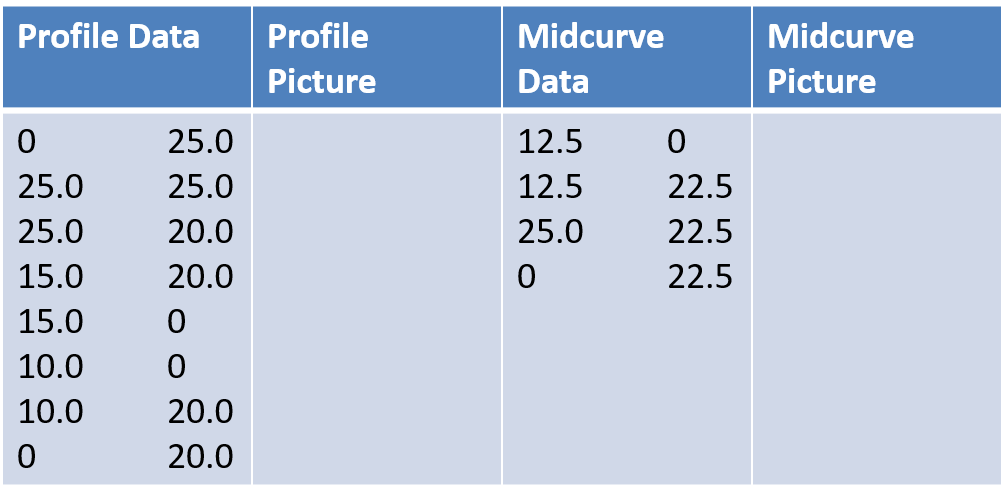
\includegraphics[width=0.9\linewidth,keepaspectratio]{midcurve28}
\end{center}

	\begin{itemize}
	\item For each shape, we have this pair of input and output. That's it. 
	\item We need to start with these few samples only
	\end{itemize}
	
\end{frame}

%%%%%%%%%%%%%%%%%%%%%%%%%%%%%%%%%%%%%%%%%%%%%%%%%%%%%%%%%%%%%%%%%%%%%%%%%%%%%%%%%%
\begin{frame}[fragile]\frametitle{Augmentation}

	\begin{itemize}
	\item Such few profile shapes, are  just not enough for Neural Networks to train.
	\item Need more with as much diversity as possible.
	\item Will need to artificially augment data with transformations, like pan, rotate, mirror, etc.
	\item All needs to be automatically, programmatically
	\end{itemize}
	
\end{frame}

%%%%%%%%%%%%%%%%%%%%%%%%%%%%%%%%%%%%%%%%%%%%%%%%%%%%%%%%%%%%%%%%%%%%%%%%%%%%%%%%%%
\begin{frame}[fragile]\frametitle{Geometry to Image}
	\begin{itemize}
	\item Raw input data is in the Vector format
	\item Converted it to fixed size $(100x100)$ image by rasterization of drawSVG library.
	\end{itemize}
\begin{center}
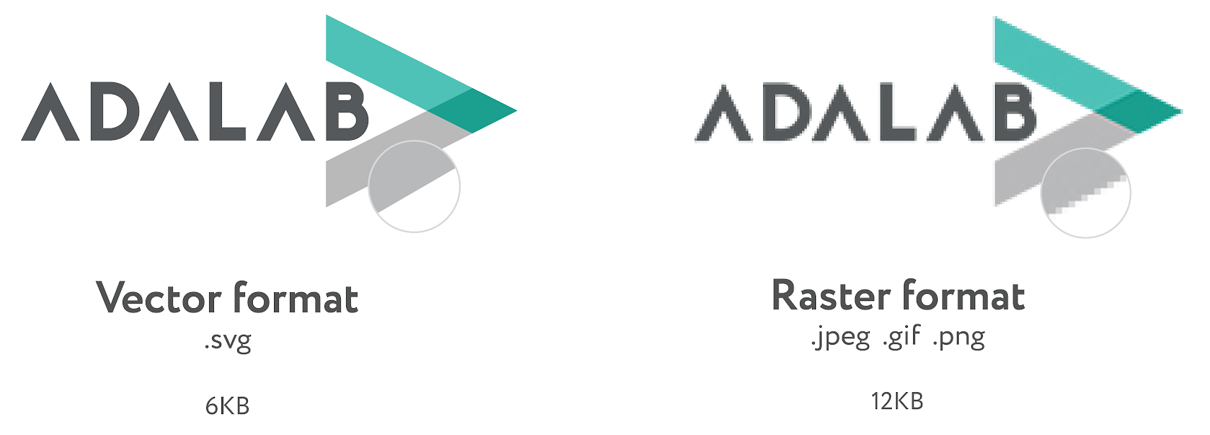
\includegraphics[width=0.9\linewidth,keepaspectratio]{midcurve29}
\end{center}	
\end{frame}

%%%%%%%%%%%%%%%%%%%%%%%%%%%%%%%%%%%%%%%%%%%%%%%%%%%%%%%%%%%%%%%%%%%%%%%%%%%%%%%%%%
\begin{frame}[fragile]\frametitle{Variations}

  \begin{columns}[t]
    \begin{column}[T]{0.4\linewidth}
      \centering
      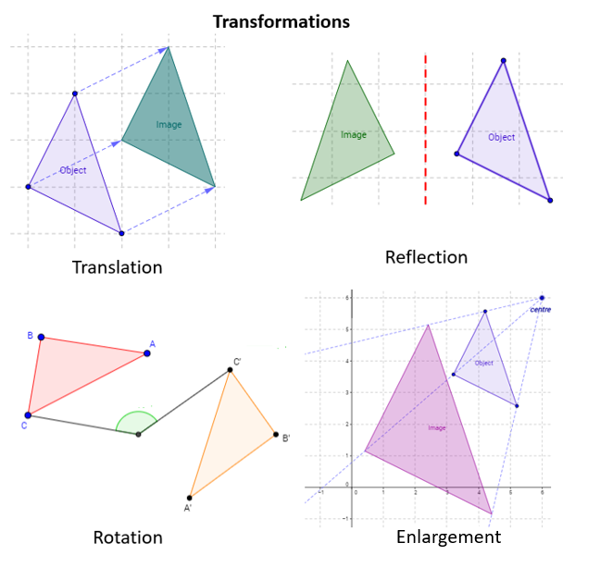
\includegraphics[width=0.9\linewidth,keepaspectratio]{midcurve30}
    \end{column}
    \begin{column}[T]{0.6\linewidth}
	\begin{itemize}
	\item Inputs: I, L, Plus, T
	\item Operations:
	\begin{itemize}
		\item Translated
		\item Rotated
		\item Mirrored
		\item Mirrored Translated
		\item Mirrored Rotated
	\end{itemize}
	\item Total: 896 images (still less, but not bad)
	\end{itemize}
    \end{column}
  \end{columns}
  \end{frame}
  
 %%%%%%%%%%%%%%%%%%%%%%%%%%%%%%%%%%%%%%%%%%%%%%%%%%%%%%%%%%%%%%%%%%%%%%%%%%%%%%%%%%
\begin{frame}[fragile]\frametitle{Training Data Samples}

\begin{center}
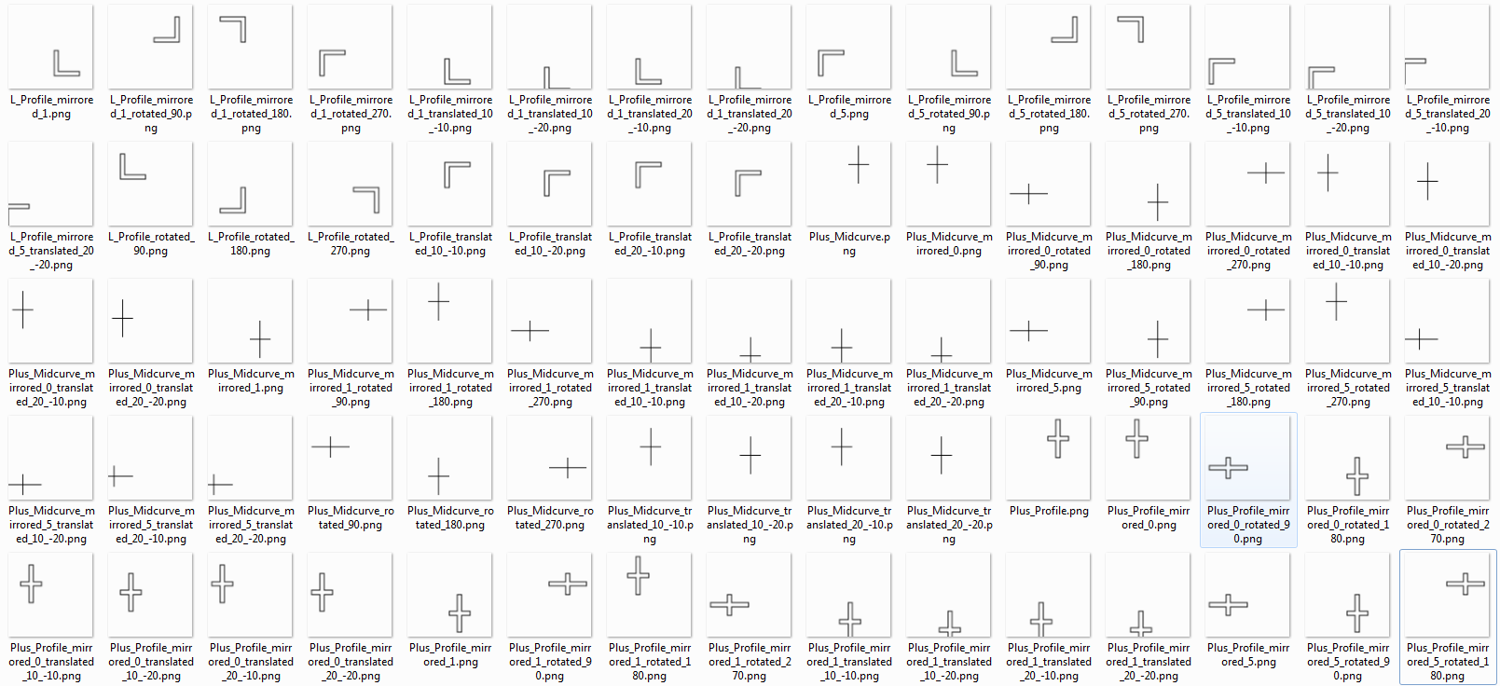
\includegraphics[width=\linewidth,keepaspectratio]{midcurve31}
\end{center}	
\end{frame}

%%%%%%%%%%%%%%%%%%%%%%%%%%%%%%%%%%%%%%%%%%%%%%%%%%%%%%%%%%%%%%%%%%%%%%%%%%%%%%%%%%
\begin{frame}[fragile]\frametitle{}
\begin{center}
{\Large Midcurve By Neural Network}
\end{center}
\end{frame}

%%%%%%%%%%%%%%%%%%%%%%%%%%%%%%%%%%%%%%%%%%%%%%%%%%%%%%%%%%%%%%%%%%%%%%%%%%%%%%%%%%
\begin{frame}[fragile]\frametitle{Options For Architectures}
	\begin{itemize}
	\item Simple Encoder Decoder (one layer each)
	\item Dense Encoder Decoder
	\item Convolutional Encoder Decoder
	\item Pix2Pix
	\item \ldots
	\end{itemize}	
\end{frame}

%%%%%%%%%%%%%%%%%%%%%%%%%%%%%%%%%%%%%%%%%%%%%%%%%%%%%%%%%%%%%%%%%%%%%%%%%%%%%%%%%%
\begin{frame}[fragile]\frametitle{}
\begin{center}
{\Large Simple Encoder Decoder}
\end{center}
\end{frame}

%%%%%%%%%%%%%%%%%%%%%%%%%%%%%%%%%%%%%%%%%%%%%%%%%%%%%%%%%%%%%%%%%%%%%%%%%%%%%%%%%%
\begin{frame}[fragile]\frametitle{Simple Encoder Decoder}

\begin{center}
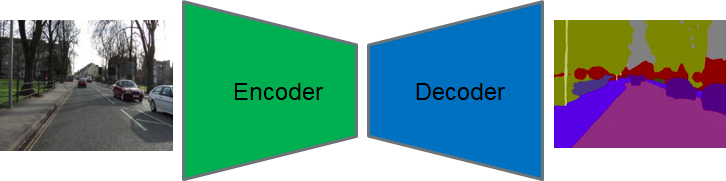
\includegraphics[width=0.9\linewidth,keepaspectratio]{midcurve32}
\end{center}	
\end{frame}

%%%%%%%%%%%%%%%%%%%%%%%%%%%%%%%%%%%%%%%%%%%%%%%%%%%%%%%%%%%%%%%%%%%%%%%%%%%%%%%%%%
\begin{frame}[fragile]\frametitle{Keras Implementation}

\begin{lstlisting}
input_img = Input(shape=(input_dim,))
    
encoded = Dense(encoding_dim, activation='relu',activity_regularizer=regularizers.l1(10e-5))(input_img)
decoded = Dense(input_dim, activation='sigmoid')(encoded) 
    
autoencoder = Model(input_img, decoded)
            
encoder = Model(input_img, encoded)
encoded_input = Input(shape=(encoding_dim,))
decoder_layer = autoencoder.layers[-1]
decoder = Model(encoded_input, decoder_layer(encoded_input))
    
autoencoder.compile(optimizer='adadelta', loss='binary_crossentropy')
\end{lstlisting}	
\end{frame}

%%%%%%%%%%%%%%%%%%%%%%%%%%%%%%%%%%%%%%%%%%%%%%%%%%%%%%%%%%%%%%%%%%%%%%%%%%%%%%%%%%
\begin{frame}[fragile]\frametitle{Results}

\begin{center}
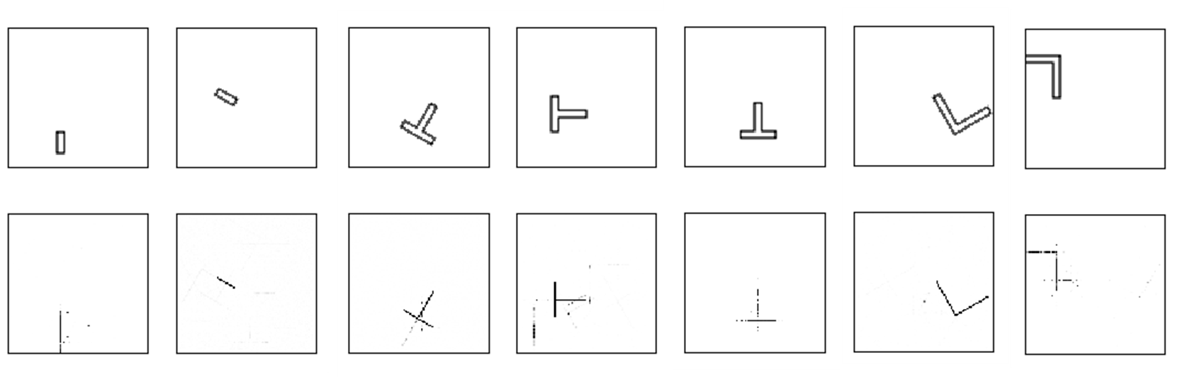
\includegraphics[width=\linewidth,keepaspectratio]{midcurve33}
\end{center}	
\end{frame}

%%%%%%%%%%%%%%%%%%%%%%%%%%%%%%%%%%%%%%%%%%%%%%%%%%%%%%%%%%%%%%%%%%%%%%%%%%%%%%%%%%
\begin{frame}[fragile]\frametitle{Results}
	\begin{itemize}
	\item Not very perfect but encouraging
	\item NN is correct with 
	\begin{itemize}
	\item The location (bounding box)
	\item Dimension Reduction is seen
	\end{itemize}	
	\item But, still some stray points and misses
	\end{itemize}	
\end{frame}

%%%%%%%%%%%%%%%%%%%%%%%%%%%%%%%%%%%%%%%%%%%%%%%%%%%%%%%%%%%%%%%%%%%%%%%%%%%%%%%%%%
\begin{frame}[fragile]\frametitle{What can be done?}
	\begin{itemize}
	\item For the noise, use bounding boxes 
	\item Feedback into error term: differencing with the known output expected 
	\item Classify single pixel image as the skeleton, and rest as noise. 
	\end{itemize}	
\end{frame}

%%%%%%%%%%%%%%%%%%%%%%%%%%%%%%%%%%%%%%%%%%%%%%%%%%%%%%%%%%%%%%%%%%%%%%%%%%%%%%%%%%
\begin{frame}[fragile]\frametitle{What Next?}
	\begin{itemize}
	\item Add denoiser network after the current one
	\item More Network Architectures
	\item Sequence-to-Sequence based approaches, taking closed thin polygon as input and polyline as output
	\item Extending to 3D, ie Midsurface
	\end{itemize}	
\end{frame}
